\documentclass[border=3pt, multi, tikz]{standalone}
\usepackage[T1]{fontenc}
\usepackage{lmodern}
\usepackage{amsmath}
\usetikzlibrary{arrows.meta,calc,positioning,fit,backgrounds}

% Soft-skeletonisation operator panel.
%
% Two things this figure exists to show, both of which are load-bearing in the text
% and neither of which is visible in the rendered-patch figure:
%   (a) the erosion and dilation neighbourhoods are NOT the same shape -- erosion is
%       the 6-neighbour cross reached by three directional minimum pools, dilation is
%       the full 3^3 cube -- so the "opening" is not an adjoint morphological pair;
%   (b) the accumulation is a recurrence with a soft union, not a single subtraction.
%
% No patient data appears here: this is operator geometry and dataflow only.

\definecolor{opFill}{HTML}{E8EEF7}
\definecolor{opEdge}{HTML}{3A5A8C}
\definecolor{cellOn}{HTML}{4C78A8}
\definecolor{cellOff}{HTML}{D9E2EF}
\definecolor{cubeFill}{HTML}{F2C57C}
\definecolor{cubeEdge}{HTML}{B07A2E}
\definecolor{accFill}{HTML}{EFE3F2}
\definecolor{accEdge}{HTML}{7B4B94}

\newcommand{\FigBody}{\fontsize{10.5}{12.0}\selectfont}
\newcommand{\FigSmall}{\fontsize{9.0}{10.5}\selectfont}

\begin{document}
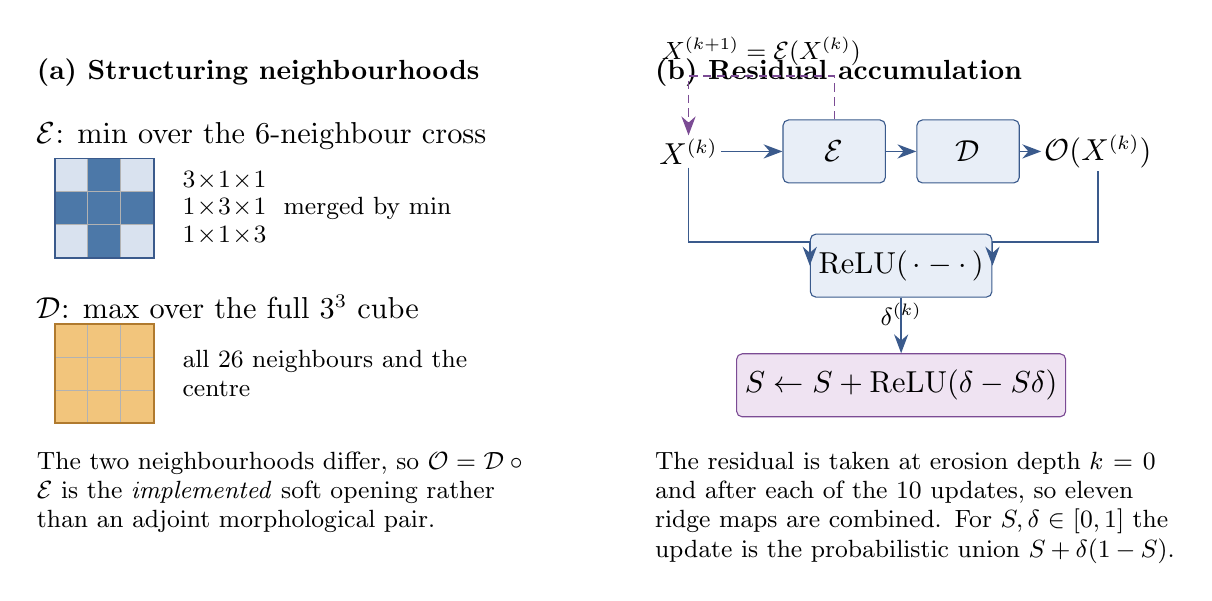
\begin{tikzpicture}[
  font=\FigBody,
  op/.style   = {draw=opEdge, fill=opFill, rounded corners=2pt, minimum height=8mm,
                 minimum width=13mm, inner sep=3pt},
  acc/.style  = {draw=accEdge, fill=accFill, rounded corners=2pt, minimum height=8mm,
                 minimum width=13mm, inner sep=3pt},
  sig/.style  = {inner sep=1pt},
  flow/.style = {-{Stealth[length=2.4mm]}, draw=opEdge, line width=0.5pt},
  loop/.style = {-{Stealth[length=2.4mm]}, draw=accEdge, line width=0.5pt, densely dashed},
]

% ---------------------------------------------------------------- (a) neighbourhoods
\begin{scope}[shift={(0,0)}]
  \node[anchor=west, font=\bfseries] at (-0.35,2.35) {(a) Structuring neighbourhoods};

  % --- erosion: the 6-neighbour cross, built from three directional min pools -------
  \node[anchor=west] at (-0.35,1.55)
    {$\mathcal{E}$: $\min$ over the $6$-neighbour cross};
  \foreach \x/\y in {1/0, 0/1, 1/1, 2/1, 1/2} {
    \fill[cellOn] (0.42*\x, 0.42*\y) rectangle ++(0.42,0.42);
  }
  \foreach \x/\y in {0/0, 2/0, 0/2, 2/2} {
    \fill[cellOff] (0.42*\x, 0.42*\y) rectangle ++(0.42,0.42);
  }
  \draw[step=0.42, gray!60, line width=0.3pt] (0,0) grid (1.26,1.26);
  \draw[opEdge, line width=0.6pt] (0,0) rectangle (1.26,1.26);
  \node[anchor=west, font=\FigSmall] at (1.5,0.98) {$3\!\times\!1\!\times\!1$};
  \node[anchor=west, font=\FigSmall] at (1.5,0.63) {$1\!\times\!3\!\times\!1$\ \ merged by $\min$};
  \node[anchor=west, font=\FigSmall] at (1.5,0.28) {$1\!\times\!1\!\times\!3$};

  % --- dilation: the full 3^3 cube --------------------------------------------------
  \node[anchor=west] at (-0.35,-0.62)
    {$\mathcal{D}$: $\max$ over the full $3^{3}$ cube};
  \foreach \x in {0,1,2} { \foreach \y in {0,1,2} {
    \fill[cubeFill] (0.42*\x, -2.1+0.42*\y) rectangle ++(0.42,0.42);
  }}
  \draw[step=0.42, gray!60, line width=0.3pt] (0,-2.1) grid (1.26,-0.84);
  \draw[cubeEdge, line width=0.6pt] (0,-2.1) rectangle (1.26,-0.84);
  \node[anchor=west, font=\FigSmall, text width=42mm] at (1.5,-1.47)
    {all $26$ neighbours and the centre};

  \node[anchor=north west, font=\FigSmall, text width=62mm, align=left] at (-0.35,-2.35)
    {The two neighbourhoods differ, so $\mathcal{O}=\mathcal{D}\circ\mathcal{E}$ is the
     \emph{implemented} soft opening rather than an adjoint morphological pair.};
\end{scope}

% ---------------------------------------------------------------- (b) recurrence
\begin{scope}[shift={(8.4,0)}]
  \node[anchor=west, font=\bfseries] at (-0.9,2.35) {(b) Residual accumulation};

  \node[sig] (xk) at (-0.35,1.35) {$X^{(k)}$};
  \node[op]  (er) at (1.5,1.35)   {$\mathcal{E}$};
  \node[op]  (di) at (3.2,1.35)   {$\mathcal{D}$};
  \node[sig] (ok) at (4.85,1.35)  {$\mathcal{O}(X^{(k)})$};

  \draw[flow] (xk) -- (er);
  \draw[flow] (er) -- (di);
  \draw[flow] (di) -- (ok);

  % residual node
  \node[op] (res) at (2.35,-0.1) {$\operatorname{ReLU}(\,\cdot-\cdot\,)$};
  \draw[flow] (xk.south) |- ([yshift=3mm]res.west) -- (res.west);
  \draw[flow] (ok.south) |- ([yshift=3mm]res.east) -- (res.east);
  \node[sig, font=\FigSmall] at (2.35,-0.72) {$\delta^{(k)}$};

  % soft union accumulator
  \node[acc] (acc) at (2.35,-1.62) {$S \leftarrow S+\operatorname{ReLU}(\delta-S\delta)$};
  \draw[flow] (res.south) -- (acc.north);

  % erosion feedback
  \draw[loop] (er.north) -- ++(0,0.55) -| node[pos=0.25, above, font=\FigSmall]
    {$X^{(k+1)}=\mathcal{E}(X^{(k)})$} (xk.north);

  \node[anchor=north west, font=\FigSmall, text width=66mm, align=left] at (-0.9,-2.35)
    {The residual is taken at erosion depth $k=0$ and after each of the $10$ updates,
     so eleven ridge maps are combined. For $S,\delta\in[0,1]$ the update is the
     probabilistic union $S+\delta(1-S)$.};
\end{scope}

\end{tikzpicture}
\end{document}
